\chapter{Demo}\label{ch:demo}

\section{Requisiti}\label{sec:demo-requisiti}

\section{Design architetturale}\label{sec:demo-design-architetturale}
A seguito dell'analisi dei requisiti definiti nella sezione precedente, si è realizzato il design architetturale di
massima riportato in Figura~TODO.

Il pattern architetturale scelto è \ECS, dato che si presta bene a questo genere di applicazioni.
Per non legarsi a una specifica libreria grafica, si è deciso d'introdurre il \textit{façade} \texttt{ECSCanvas}
che espone dei metodi di alto livello per disegnare le primitive richieste (in particolare, cerchio e linea) e ottenere
le dimensioni dell'area di disegno.

\section{Design di dettaglio}\label{sec:demo-design-di-dettaglio}

Si elencano di seguito i sistemi individuati ai fini della realizzazione della demo:
\begin{itemize}
    \item \textbf{CollisionSystem}: calcola le nuove velocità di eventuali entità che collidono fra loro
\end{itemize}

\section{Implementazione}\label{sec:demo-implementazione}

Di seguito si riportano gli aspetti implementativi che meritano una trattazione più approfondita.

\subsection{Di Domenico}\label{subsec:demo-di-domenico}

\subsubsection{Collision System}
Il sistema principale che gestisce la simulazione è il \texttt{CollisionSystem}: questo implementa i calcoli necessari
per testare se c'è una collisione fra due corpi e, in caso affermativo, calcolarne le nuove velocità.

Sarebbe necessario controllare tutte le possibili coppie di corpi, ma questo presenta due importanti problemi:
\begin{itemize}
    \item ogni coppia di entità compare due volte anziché una
    \item la gran parte delle coppie di entità non porterà a una collisione, essendo troppo distanti fra loro
\end{itemize}

La soluzione a entrambi questi problemi è stata quella di applicare la tecnica di ottimizzazione detta
\textit{space partitioning}: si divide lo spazio (il piano in questo caso, essendo una simulazione 2D) in regioni disgiunte
affinché ogni entità appartenga a una e una sola di esse.
Per fare ciò è stato creato il concetto di \texttt{SpacePartitionContainer}, che prende in ingresso un'entità con
tutti i componenti richiesti e la salva in una mappa che associa ogni regione (identificata da una coppia di numeri interi)
alla lista di entità che ne fanno parte.
Inoltre, lo \texttt{SpacePartitionContainer} dispone di un metodo per ottenere tutte le entità facente parte di una regione
specificata, e uno per iterare su tutte le regioni non vuote.

A questo punto, il \texttt{CollisionSystem} può diventare molto più efficiente: ora è sufficiente iterare su tutte le regioni
non vuote e testare le collisioni solo fra entità che fanno parte di un intorno bidimensionale di quelle regioni, come
mostrato in Figura~\ref{fig:space-partition}.
Per non processare due volte le coppie di entità, si costruiscono tutte le possibili combinazioni di lunghezza 2 e si
considera solo una metà dell'intorno, mentre l'altra verrà coperta nelle successive iterazioni delle regioni non vuote.

\begin{figure}[htp]
    \centering
    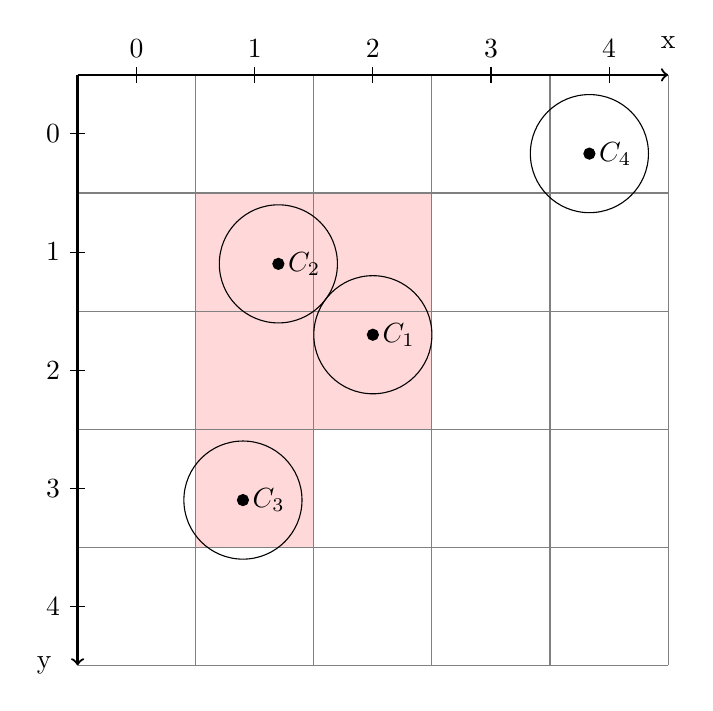
\begin{tikzpicture}
        \fill[red!15!white] (1.5, 6) rectangle (4.5, 3);
        \fill[red!15!white] (1.5, 3) rectangle (3, 1.5);
        \draw[step=1.5cm,gray,thin] (0, 0) grid (7.5, 7.5);
        \draw[thick,->] (0, 7.5) -- (7.5, 7.5) node[above=2mm] {x};
        \draw[thick,->] (0, 7.5) -- (0, 0) node[left=2mm] {y};
        \foreach \x [count=\i from 0] in {0, 1.5, 3, 4.5, 6}
            \draw (0.75+\x, 7.6) -- (0.75+\x, 7.4) node[above=2mm]{$\i$};
        \foreach \y [count=\i from 0] in {0, 1.5, 3, 4.5, 6}
            \draw (-0.1, 6.75-\y) -- (0.1, 6.75-\y) node[left=2mm]{$\i$};
        \draw (3.75, 4.2) circle (0.75cm);
        \filldraw[black] (3.75, 4.2) circle (2pt) node[anchor=west]{$C_1$};
        \draw (2.55, 5.1) circle (0.75cm);
        \filldraw[black] (2.55, 5.1) circle (2pt) node[anchor=west]{$C_2$};
        \draw (2.1, 2.1) circle (0.75cm);
        \filldraw[black] (2.1, 2.1) circle (2pt) node[anchor=west]{$C_3$};
        \draw (6.5, 6.5) circle (0.75cm);
        \filldraw[black] (6.5, 6.5) circle (2pt) node[anchor=west]{$C_4$};
    \end{tikzpicture}
    \caption{La regione in esame $(2, 2)$ controllerà solo se c'è collisione fra i cerchi con centro nelle regioni limitrofe (l'area rossa);
    si considera solo metà intorno per non contare due volte le coppie nelle iterazioni successive;
    si testerà quindi la collisione fra $C_1$ e $C_2$ e fra $C_1$ e $C_3$, mentre $C_4$ non viene preso in considerazione.}
    \label{fig:space-partition}
\end{figure}
